\documentclass{lab}

\usepackage{graphicx}
\usepackage{float}
\usepackage{soul}
\usepackage{multicol}

\addtolength{\oddsidemargin}{-.4in}
\addtolength{\evensidemargin}{-.4in}

\title{ENGG1003 - Lab Week 5}
\author{Brenton Schulz}
\date{\today}

\begin{document}
\maketitle

\section{Pre-Reading}
Read through the following textbook sections:

\begin{itemize}
\item Section 2.4 Random Numbers: \url{https://link.springer.com/chapter/10.1007/978-3-030-16877-3_2#Sec23}
\item Section 3.3.4 Example: Random Walk in Two Dimensions: \url{https://link.springer.com/chapter/10.1007/978-3-030-16877-3_3#Sec10}
\end{itemize}

\pagebreak

\section{Revision - Summations and \texttt{for} Loops}

The Week 3 lab included Exercise 3.11 from the textbook. This exercise requires an ``infinite sum'' to be evaluated of the form:

\begin{equation}\label{eq:pi}
\pi = 8 \sum_{k=0}^{\infty}\frac{1}{(4k+1)(4k+3)}
\end{equation}

Breaking down this notation:
\begin{itemize}
\item $\Sigma$ means ``sum''
\item $k=0$ below the $\Sigma$ means that $k$ is a \textit{variable} which takes integer values starting at zero
\item $\infty$ above the $\Sigma$ means that there is no limit to how large $k$ can become
\item Each value of $k$ gets substituted into the $\frac{1}{(4k+1)(4k+3)}$ expression and all results added together
\item ``$\pi=$'' implies that the sum will approach $\pi$ as $k$ approaches $\infty$
\end{itemize}

Putting it all together, the first few terms of Equation \ref{eq:pi} can be written out as:

\begin{equation}
\frac{1}{(4\times 0 + 1)(4 \times 0 + 3)} + \frac{1}{(4\times 1 + 1)(4 \times 1 + 3)} + \frac{1}{(4\times 2 + 1)(4 \times 2 + 3)} + ...
\end{equation}

It turns out that expressions of this form map quite cleanly to \texttt{for} loops when programming:

\begin{itemize}
\item An expression is evaluated multiple times for different values of one variable
\item A \texttt{sum} variable can ``accumulate'' calculations inside the loop in the form \texttt{sum = sum + <something>}
\item $k$ as the ``summation variable'' becomes the ``loop variable'' \texttt{k}
	\begin{itemize}
		\item Pay close attention to the starting value of \texttt{k=0}
		\item Computer's can't count to $\infty$, so choose a ``reasonable'' value of, say, 100 000 for the final value of \texttt{k}
	\end{itemize}
\item The $\frac{1}{(4k+1)(4k+3)}$ expression becomes the Python expression \texttt{1/((4*k+1)*(4*k+3))} (note double level nesting of \texttt{( ()() )} in the denominator - without the outer \texttt{( )} the expression becomes $\frac{4k+3}{4k+1}$.
\end{itemize}

\begin{task}{Python Implementation of Equation \ref{eq:pi}}{}
Given all the above, write a Python script which implements Equation \ref{eq:pi} for \texttt{k=0} to \texttt{k=99} (ie: with \texttt{range(0,100)}.
\\~\\
Remember to multiply the result of the summation by 8 to get an approximation of $\pi$!
\\~\\
The final value should be \texttt{3.13659}.
\\~\\
If you get \texttt{0.39207} the multiply by 8 was omitted.
\\~\\
Once your code is correct repeat the calculation with \texttt{range(0,100000)} to get the more accurate result of \texttt{3.141587}.
\end{task}

\pagebreak
\section{Random Numbers}
\begin{task}{Simplified Random Walk}{}
Section 3.3.4 of the textbook shows a ``random walk'' program which randomly moves a point N, S, E, or W 1000 times.
\\~\\
In this task you will repeat this problem with floating point steps. ie: the x and y movements will be drawn from a uniform distribution using \texttt{np.random.uniform()}. This will make the simulation roughly analogous to brownian motion - the movement of particles in a liquid or gas.
\\~\\
The program is to fill in two \texttt{numpy} arrays: one of x locations and one of y. The array index will then become a ``time'' variable. This will allow the simulation results to be plotted with \texttt{plot(x,y)}.
\\~\\
Write a Python script which implements the follow pseudocode to move a point around randomly and plot the result:
\begin{lstlisting}
BEGIN
	N = 1000
	x = an array of N zeros
	y = an array of N zeros
	FOR each element, n, in x and y from 1 to N:
		x[n] = x[n-1] + a random float from [-1,1)
		y[n] = y[n-1] + a random float from [-1,1)
	ENDFOR
	plot the set of x-y points, drawing lines between points
END
\end{lstlisting}
You may call \texttt{np.random.uniform()} within the loop or create a pair of additional arrays containing random numbers before entering the loop.
\end{task}

\pagebreak
\section{The CSV Format}

As seen in lectures, we will be studying the use of the \texttt{pandas} library for reading CSV (comma separated value/variable) files.

The CSV format allows for ``spreadsheet'' data to be stored as ``human-readable'' ASCII text. Column headings and numerical values are written as plain text and columns are separated by commas\footnote{Some variations allow for space or tab separation while still being classed as ``CSV'' files.}. Rows are separated by new lines.

\begin{task}{Opening CSV Files}{}
This lab will make use of a real scientific dataset from the Bureau of Meteorology. The Bureau of Meteorology makes a vast amount of climate data available online here: \url{http://www.bom.gov.au/climate/data/index.shtml}
\\~\\
You are welcome to browse data as it suits your interest but this lab will make use of the monthly rainfall data for the Nobbys Signal Station weather station on the coast of Newcastle.
\\~\\
The data used in this lab (see \texttt{rainfall-1.csv} on Blackboard) has been extracted from the monthly rainfall data for Nobbys Signal Station AWS.
\\~\\
Download \textbf{rainfall-1.csv} from Blackboard and open it in a \textbf{text editor}. The lab computers have Notepad++ installed but you could also use Notepad or, at worst, open them in PyCharm.
\\~\\
Observe the ``human readable'' nature of the \texttt{csv} format. You may wish to keep this file open for debugging purposes.
\\~\\
Note that the data provided by the BOM has several gaps. To simplify this week's task the \texttt{rainfall-1.csv} file only contains a \textit{subset} of the full rainfall history from the Nobbys weather station.
\end{task}

In this course we will use the \texttt{pandas} library to read \texttt{csv} files. Before it can be used you must run \texttt{pip install pandas} to install it.

\pagebreak
\begin{task}{Reading and Analysing Rainfall Data}{}
This task is presented in multiple parts and is presented in a more ``real'' style compared to previous lab tasks. You are welcome to discuss problem solving strategies with your lab peers as well as demonstrators.
\\~\\
Background lecture material: \\~\\
See Slide 18f of the Thursday Week 4 lecture slides for a \texttt{pandas} example. The recording timestamp is: \url{https://www.youtube.com/watch?v=GZmJTGqh5pw#t=50m45s}\\
\begin{enumerate}
\item \textbf{Download \texttt{rainfall-1.csv} from Blackboard}.
\item To open this file with \texttt{pandas} you must either:
\begin{itemize}
\item Copy \texttt{rainfall-1.csv} to the same folder as your \texttt{.py} script file
	\begin{itemize}
		\item You can get the project's folder by right clicking on the ``tab'' for a \texttt{.py} file and selecting ``Open in -> Explorer''
		\item You can also drag \& drop the \texttt{.csv} file to the project,  dropping it over the ``top level'' project name.
\begin{figure}[H]
\begin{center}
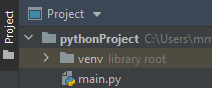
\includegraphics[width=0.4\textwidth]{Wk5Figs/project.png}
\end{center}
\caption{Drag and drop \texttt{rainfall-1.csv} to ``pythonProject''.}
\end{figure}

	\end{itemize}
\item Reference it with an absolute file path. The complication with this method is that the \texttt{\textbackslash} character, when used in a Python string, indicates an ``escape sequence''. For example \texttt{\textbackslash n} is a special character which prints a new line.
\\~\\
As such, the \texttt{\textbackslash} characters in the file path need to be ``escaped'' by placing an \textit{additional} \texttt{\textbackslash} before them. eg: \texttt{C:\textbackslash\textbackslash Users\textbackslash \textbackslash me\textbackslash \textbackslash Downloads\textbackslash \textbackslash rainfall-1.csv}.
\end{itemize}
\item Write a Python script which uses \texttt{pandas} to open \texttt{rainfall-1.csv} and use the \texttt{head()} function to print the first few lines. Ensure that they match what you saw in the text editor during the previous task.
\item Extend your script to load rainfall data from \texttt{rainfall-1.csv} into a single \texttt{numpy} array called \texttt{rainfall}.
\\~\\
Your array should be 1584 elements. Data is provided from Janurary 1867 to December 1998.
\\~\\
Observe the first line of the file to work out the correct column heading.
\item Plot the timeseries data. A simple \texttt{plot(rainfall)} will suffice here as we are visualising the data for development purposes - not producing a plot for publication.

\item Summary statistics for Nobbys Signal Station are provided by the BOM at the bottom of this page: \url{http://www.bom.gov.au/jsp/ncc/cdio/weatherData/av?p_nccObsCode=139&p_display_type=dataFile&p_startYear=&p_c=&p_stn_num=061055}
\\~\\
From data in the \texttt{rainfall} array calculate the mean, lowest, and highest rainfall figures for each month and compare them with the BOM's calculations. Use one (or more) \texttt{for} loops to perform this analysis.
\\~\\
Your calculations won't be exactly the same as the BOM data because \texttt{rainfall-1.csv} is a subset of the full rainfall \texttt{csv} file. You can, however, use the summary statistics as a rough guide to judge if your calculations are correct or not.
\\~\\
Note that the \texttt{\%} (modulus) operator may be useful when converting an array index to a month. ie: the index modulo 12 will provide a month number where 0 is Janurary and 11 is December.
\\~\\
Alternatively, you can write one or more \texttt{for} loops which count in increments of 12 to ``pick out'' all values from a given month. Starting from index 0 and counting by 12s will provide all January data. Starting from index 1 will pick out all February data, etc.
\\~\\
It is simpler to complete this task with twelve variables (ie: one running sum for each month) but an attempt should be made to solve this problem with two \textit{nested} \texttt{for} loops: an outer loop which counts months and an inner loop which tests every index for inclusion in that month. The nested loop method allows for the use of an array to store the monthly means and greatly reduces the code complexity.

\item \textbf{Extension:} Plot a \textit{histogram} of the monthly rainfall data. To do this you can use the \texttt{plt.hist()} function from \texttt{matplotlib.pyplot}. If the data is stored in the \texttt{numpy} array \texttt{rainfall} then the histogram can be plotted with:

\begin{lstlisting}
plt.hist(rainfall)
plt.show()
\end{lstlisting}

\end{enumerate}
\end{task}


\end{document}
